\section{NAT}

\begin{bonus}{Konfiguration von IPv4-Adressen}
    \emph{IPv4-Adressen} müssen in jedem Endgerät, Router und sonstigen Netzwerkkomponenten konfiguriert werden.

    Jeder Knoten muss folgende Daten besitzen:
    \begin{itemize}
        \item IP und Netzwerkmaske
        \item Standard-Gateway
        \item DNS-Server
    \end{itemize}

    Grundsätzlich existieren zwei Möglichkeiten dazu:
    \begin{itemize}
        \item Manuelle Konfiguration
        \item Konfiguration über ein Protokoll (z. B. DHCP)
    \end{itemize}
\end{bonus}

\begin{bonus}{Probleme IPv4}
    Wir hatten bereits geklärt, dass IPv4 nur $2^{32}$ IP-Adressen zur Verfügung hat.

    Da bereits relativ zeitnah nach dem Anpassen der Subnetzgrößen klar wurde, dass die gewonnene Anzahl der daraus resultieren IP-Adressen nicht ausreicht, hat man sich eine provisorische Lösung überlegt.
\end{bonus}

\begin{defi}{NAT}
    \emph{NAT} (Network Adress Translation) verfolgt die Idee, dass KundInnen jeweils lediglich eine eindeutige öffentliche IPv4-Adresse erhalten.
    Dementsprechend existiert für jedes Netz ebenfalls nur einen Zugangspunkt (Gateway) zu diesem Netz.
    Das Gateway hat dabei mindestens 2 Netzwerkkarten, um in das große Internet, sowie das lokale Netz zu senden.

    Das private Netz hat nutzt meist einen der folgenden IP-Adressblöcke:\\
    \begin{tabular}{llcl}
        \texttt{10.0.0.0/8:}     & \texttt{10.0.0.0}    & - & \texttt{10.255.255.255}  \\
        \texttt{172.16.0.0/12:}  & \texttt{172.16.0.0}  & - & \texttt{172.31.255.255}  \\
        \texttt{192.168.0.0/16:} & \texttt{192.168.0.0} & - & \texttt{192.168.255.255}
    \end{tabular}
\end{defi}

\begin{example}{NAT}
    \begin{center}
        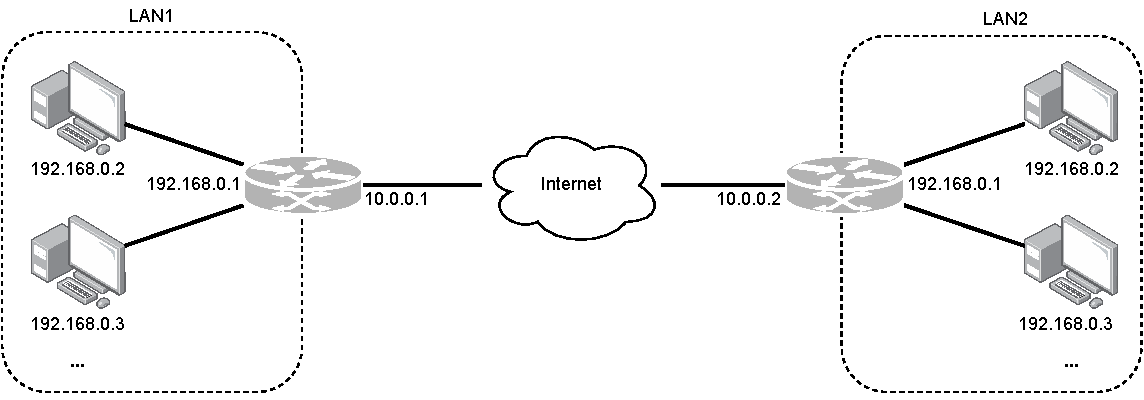
\includegraphics[width=0.75\textwidth]{includes/figures/defi_nat.pdf}
    \end{center}

    In diesem Beispiel \enquote{verbrauchen} wir 2 globale IP-Adressen, können jedoch bis zu $(2^{16} - 3)$ Adressen in jeweils 2 Netzen anbinden.
\end{example}

\begin{defi}{Adressübersetzung (NAT)}
    Zur Identifikation des Absenders bzw. Empfängers müssen im IP-Header freie Felder gefunden werden.
    Im IP-Header steht jedoch nur noch 1 freies Bit zur Verfügung.

    \begin{center}
        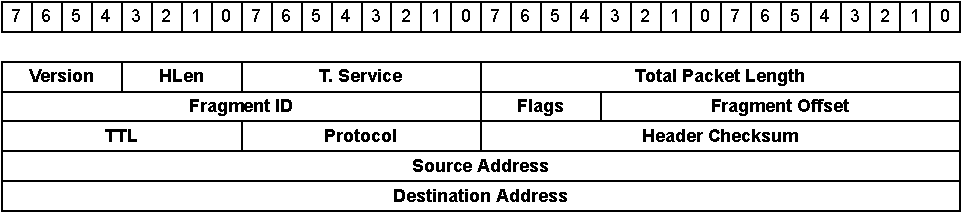
\includegraphics[width=0.75\textwidth]{includes/figures/defi_ip_header.pdf}
    \end{center}

    Zweite Idee: Nutze TCP bzw UDP Header.
    Hier kann man die 16 bit Portnummern nutzen um Clients eindeutig zu Adressieren.
    Hierbei wird jedoch die Schichten Architektur verletzt, da Layer 3 Details über Layer 4 hat.

    \begin{center}
        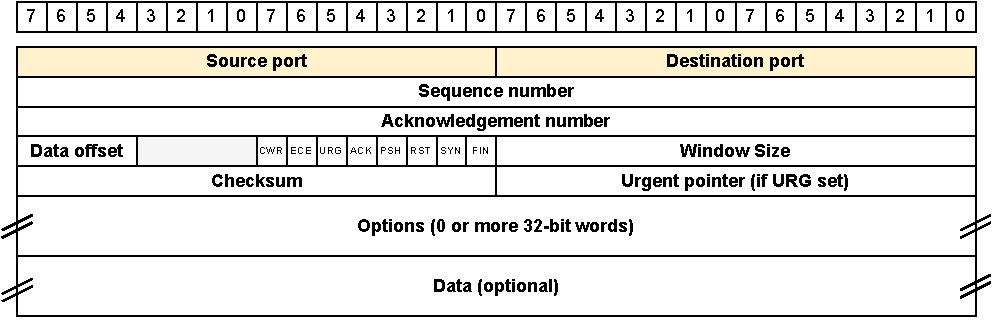
\includegraphics[width=0.75\textwidth]{includes/figures/defi_tcp_header_port.pdf}

        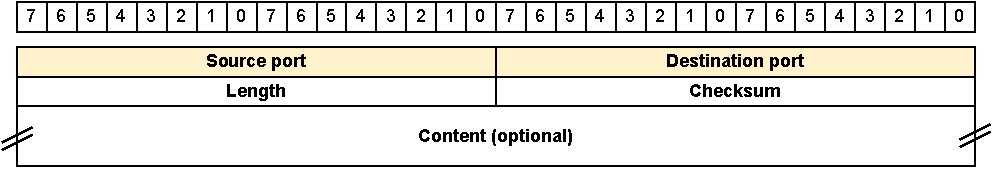
\includegraphics[width=0.75\textwidth]{includes/figures/defi_udp_header_port.pdf}
    \end{center}

    Bei TCP bzw. UDP wird sowohl der Destination Port als auch der Source Port mitgesendet.
    Der \emph{Destination Port} darf dabei von der sendenden Anwendung nicht verändert werden, da er definiert auf welchen Service Zugegriffen wird.
    Der \emph{Source Port} wird von Betriebssystem vergeben und ist ggf. nicht eindeutig (z. B. zwei Webserver mit jeweils Port \texttt{443}).

    Daher ersetzen Nat-Router den Source Port durch eine ID, die den privaten Rechner bzw. die Verbindung identifiziert.

    Im Antwortpaket muss der Destination Port extrahiert werden, und der NAT Router ersetzt die Ziel-IP mit der entsprechenden privaten IP und den Zielport mit dem ursprünglichen Port.
\end{defi}

\begin{example}{Adressübersetzung (NAT)}
    In folgendem Beispiel sendet der Rechner \texttt{192.168.0.2} in \texttt{LAN1} über den Port \texttt{4} ein Paket an den Rechner \texttt{192.168.0.2} in \texttt{LAN2} an den Port \texttt{22}.
    Dieser \enquote{versteckt} sich jedoch hinter dem öffentlichen Router \texttt{10.0.0.2} und dem Port \texttt{7000}.

    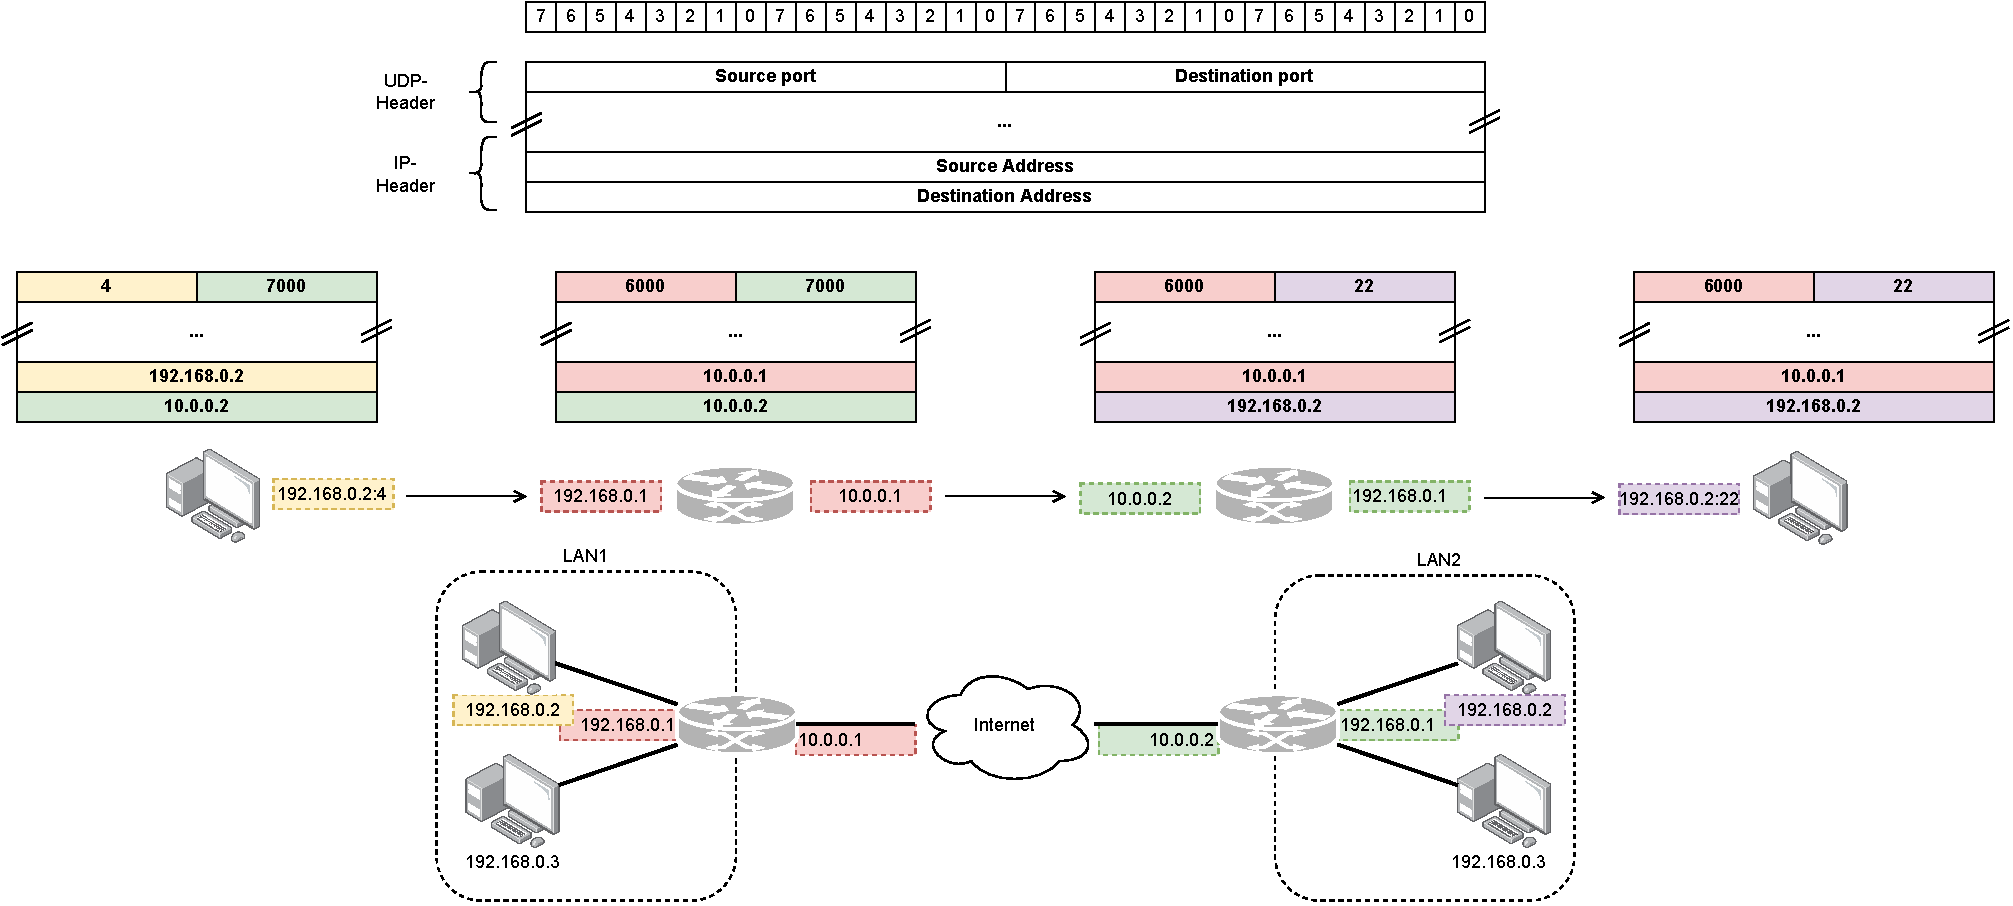
\includegraphics[width=\textwidth]{includes/figures/example_nat.pdf}

    \begin{minipage}[t]{0.5\textwidth}
        \begin{center}
            \emph{Übersetzungstabelle Router (10.0.0.2)}

            \begin{tabular}{|c|c||c|}
                \hline
                IP-Adresse  & Port & NAT-Port \\\hline\hline
                192.168.0.2 & 4    & 6000     \\\hline
                192.168.0.2 & 591  & 6001     \\\hline
                192.168.0.3 & 4    & 6002     \\\hline
            \end{tabular}
        \end{center}
    \end{minipage}
    \begin{minipage}[t]{0.5\textwidth}
        \begin{center}
            \emph{Übersetzungstabelle Router (10.0.0.2)}

            \begin{tabular}{|c|c||c|}
                \hline
                IP-Adresse  & Port & NAT-Port \\\hline\hline
                192.168.0.2 & 22   & 7000     \\\hline
                192.168.0.3 & 22   & 7001     \\\hline
            \end{tabular}
        \end{center}
    \end{minipage}
\end{example}

\begin{bonus}{NAT Nachteile}
    \begin{itemize}
        \item Nicht jeder Rechner ist eindeutig per IP identifizierbar
        \item Verletzung des Schichtenmodells
        \item Übersetzungstabelle kann i. d. R. nur aufgebaut werden, wenn ein interner Knoten die Kommunikation initiiert
        \item Was ist, wenn nicht \emph{TCP} oder \texttt{UDP} verwendet wird?
        \item Was passiert, wenn übergeordnete Protokolle die IP als Payload übertragen?
        \item Was passiert bei verschlüsselten Verbindungen?
    \end{itemize}
\end{bonus}

\begin{bonus}{Sicherheitsstufen (NAT)}
    NAT kennt unterschiedliche \emph{Sicherheitsstufen}:
    \begin{itemize}
        \item \emph{Full Cone NAT}:

              Ein Port wird unbegrenzt nach au0en freigegeben.
              Dadurch kann auch von außen ein Rechner die Kommunikation initiieren.
        \item \emph{Restricted Cone NAT}:

              Ein Port wird nur nach dem Start der internen Kommunikation freigegeben.
              Die Quell-IP-Adresse wird bei Antworten überprüft.
        \item \emph{Port Restricted Cone NAT}:

              Die Rückpakete werden zusätzlich auf den Source Port hin überprüft
    \end{itemize}
\end{bonus}

\begin{bonus}{Full Cone NAT}
    \begin{center}
        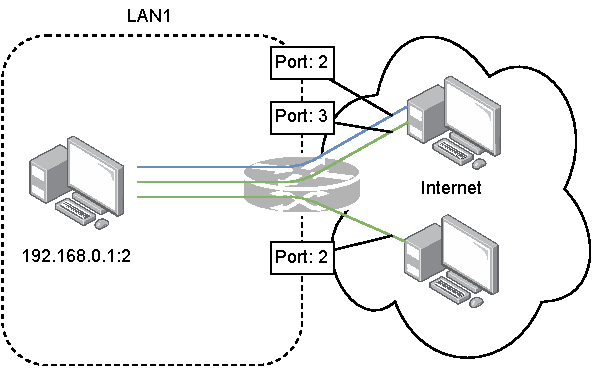
\includegraphics[width=0.75\textwidth]{includes/figures/bonus_full_cone_nat.pdf}
    \end{center}
\end{bonus}

\begin{bonus}{Restricted Cone NAT}
    \begin{center}
        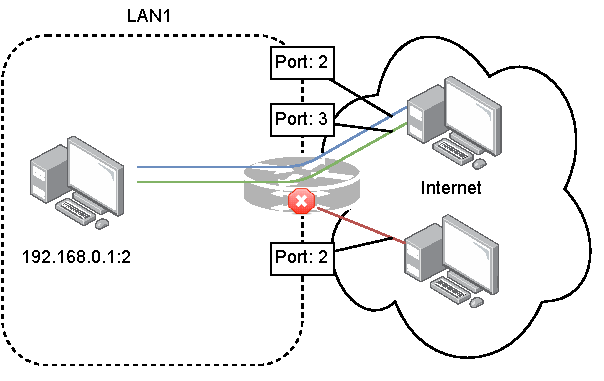
\includegraphics[width=0.75\textwidth]{includes/figures/bonus_restricted_cone_nat.pdf}
    \end{center}
\end{bonus}

\begin{bonus}{Port Restricted Cone NAT}
    \begin{center}
        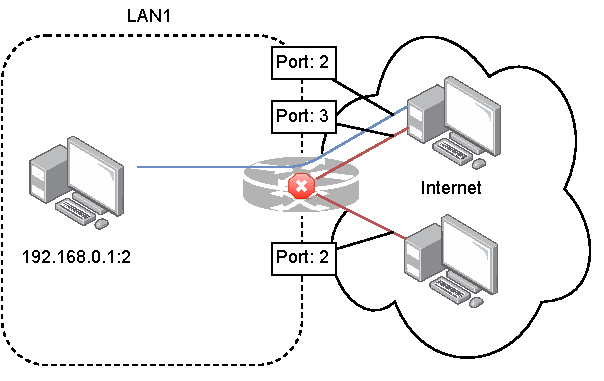
\includegraphics[width=0.75\textwidth]{includes/figures/bonus_port_restricted_cone_nat.pdf}
    \end{center}
\end{bonus}

\begin{bonus}{Symmetric NAT}
    Beim \emph{Symmetric NAT} wird für jeden Datenstrom aus dem internen Netz eine eigene Abbildung durchgeführt.
    Wenn der Quell-Rechner z. B. vom selben Quell-Port aus mit zwei unterschiedlichen Ziel-Rechnern kommuniziert, wird für jede Verbindung eine eigene NAT-Tabelle angelegt.
    Nut der jeweilige Zielrechner darf jeweils mit den eingetragenen Portnummern antworten.
\end{bonus}